The satellite is simulated using the following Python code.
\lstinputlisting[language=Python, caption=satelliteSim.py]{../control_book_public_solutions/_C_satellite/python/hw13/satelliteSim.py}
Note in line~43, that the input to the controller is the output $y$ corrupted by noise $n$ and that the input disturbance $d$ has been added to $u$ in line~44.  The dataPlotObserver plots the state $x$ and the estimated state $\hat{x}$, as well as the disturbance $d$ and estimated disturbance $\hat{d}$ which will be discussed in the next chapter.  

A Python class that implements observer-based control with an integrator for the satellite is shown below.
\lstinputlisting[language=Python, caption=satelliteController.py]{../control_book_public_solutions/_C_satellite/python/hw13/satelliteController.py}
The observer is updated on line~26, and $\hat{x}$ is used in the controller instead of $x$ but otherwise is identical to the controller in Chapter~\ref{chap:state-feedback-integrator}.  The observer is updated on lines~41--49 using the RK4 algorithm.  The differential equations for the observer are specified on lines~51--57.  

Python code that computes the observer and control gains is given below.
\lstinputlisting[language=Python, caption=satelliteParamHW13.py]{../control_book_public_solutions/_C_satellite/python/hw13/satelliteParamHW13.py}

Complete simulation code for Matlab, Python, and Simulink can be downloaded at \controlbookurl{http://controlbook.byu.edu}.

%
%A high-level Simulink diagram that implements the observer based controller using output feedback is shown in Figure~\ref{fig:hw13_simulink_satellite}.
%\begin{figure}[hbt]
%	\centering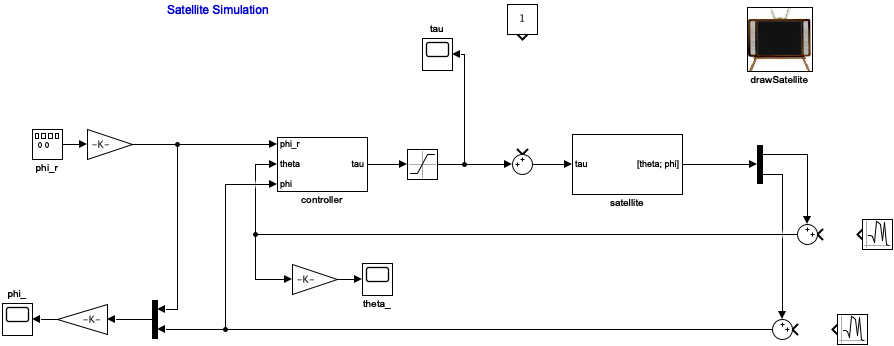
\includegraphics[width=0.8\textwidth]{6_design_studies/figures/hw13_simulink_satellite}
%	\caption{High level simulink diagram used for HW C.13}
%	\label{fig:hw13_simulink_satellite} 
%\end{figure}
%The Matlab/Simulink code for the controller is listed below.
%\lstinputlisting[language=Matlab, caption=satellite\_ctrl.m]{../control_book_public_solutions/_C_satellite/simulink/hw13/satellite_ctrl.m}
%The observer is updated on line~10, and $\hat{x}$ is used in the controller instead of $x$ but otherwise is identical to the controller in Chapter~\ref{chap:state-feedback-integrator}.  The observer is updated on lines~38--50 using the RK4 algorithm.  The differential equations for the observer are specified on lines~52--56.  
%
%Matlab code that computes the control gains is given below.
%\lstinputlisting[language=Matlab, caption=satelliteParamHW13.m]{../control_book_public_solutions/_C_satellite/simulink/hw13/satelliteParamHW13.m}
%Complete simulation code for Matlab, Python, and Simulink can be downloaded at \controlbookurl{http://controlbook.byu.edu}.
%
%The inverted pendulum is simulated using the following Python code.
%\lstinputlisting[language=Python, caption=pendulumSim.py]{../control_book_public_solutions/_B_pendulum/python/hw13/pendulumSim.py}
%Note in line~38, that the input to the controller is the output $y$ corrupted by noise $n$ and that the input disturbance $d$ has been added to $u$ in line~39.  The dataPlotObserver plots the state $x$ and the estimated state $\hat{x}$, as well as the disturbance $d$ and estimated disturbance $\hat{d}$, as will be discussed in the next chapter.  